%Template by Mark Jervelund - 2015 - mjerv15@student.sdu.dk

\documentclass[a4paper,10pt,titlepage]{report}

\usepackage[utf8]{inputenc}
\usepackage[T1]{fontenc}
\usepackage[english]{babel}
\usepackage{amssymb}
\usepackage{amsmath}
\usepackage{amsthm}
\usepackage{graphicx}
\usepackage{fancyhdr}
\usepackage{lastpage}
\usepackage{listings}
\usepackage{algorithm}
\usepackage{algpseudocode}
\usepackage[document]{ragged2e}
\usepackage[margin=1in]{geometry}
\usepackage{enumitem}
\usepackage{color}
\usepackage{datenumber}
\usepackage{venndiagram}
\usepackage{chngcntr}
\setdatetoday
\addtocounter{datenumber}{0} %date for dilierry standard is today
\setdatebynumber{\thedatenumber}
\date{}
\setcounter{secnumdepth}{0}
\pagestyle{fancy}
\fancyhf{}


%lstlisting ting:
\definecolor{dkgreen}{rgb}{0,0.45,0}
\definecolor{gray}{rgb}{0.5,0.5,0.5}
\definecolor{mauve}{rgb}{0.30,0,0.30}
\lstset{frame=tb,
  language=C++,
  aboveskip=3mm,
  belowskip=3mm,
  showstringspaces=false,
  columns=flexible,
  basicstyle={\small\ttfamily},
  numbers=left,
  numberstyle=\footnotesize,
  keywordstyle=\color{dkgreen}\bfseries,
  commentstyle=\color{dkgreen},
  stringstyle=\color{mauve},
  frame=single,
  breaklines=true,
  breakatwhitespace=false
  tabsize=1
}
\renewcommand{\lstlistingname}{Code} 

\newcommand{\Z}{\mathbb{Z}}
\lhead{Parallel Computinge (DM818))}
\rhead{Mark Jervelund (Mjerv15)}
\rfoot{Page  \thepage \, of \pageref{LastPage}}
\counterwithin*{equation}{section}

\begin{document}
\begin{titlepage}
\centering
    \vspace*{9\baselineskip}
    \huge
    \bfseries
    2. Mandatory Assignment \\
    \normalfont
    Mark Jervelund  \\
    (Mjerv15) \\
	\huge    
    Parallel Computing (DM818)  \\[4\baselineskip]
    \normalfont
	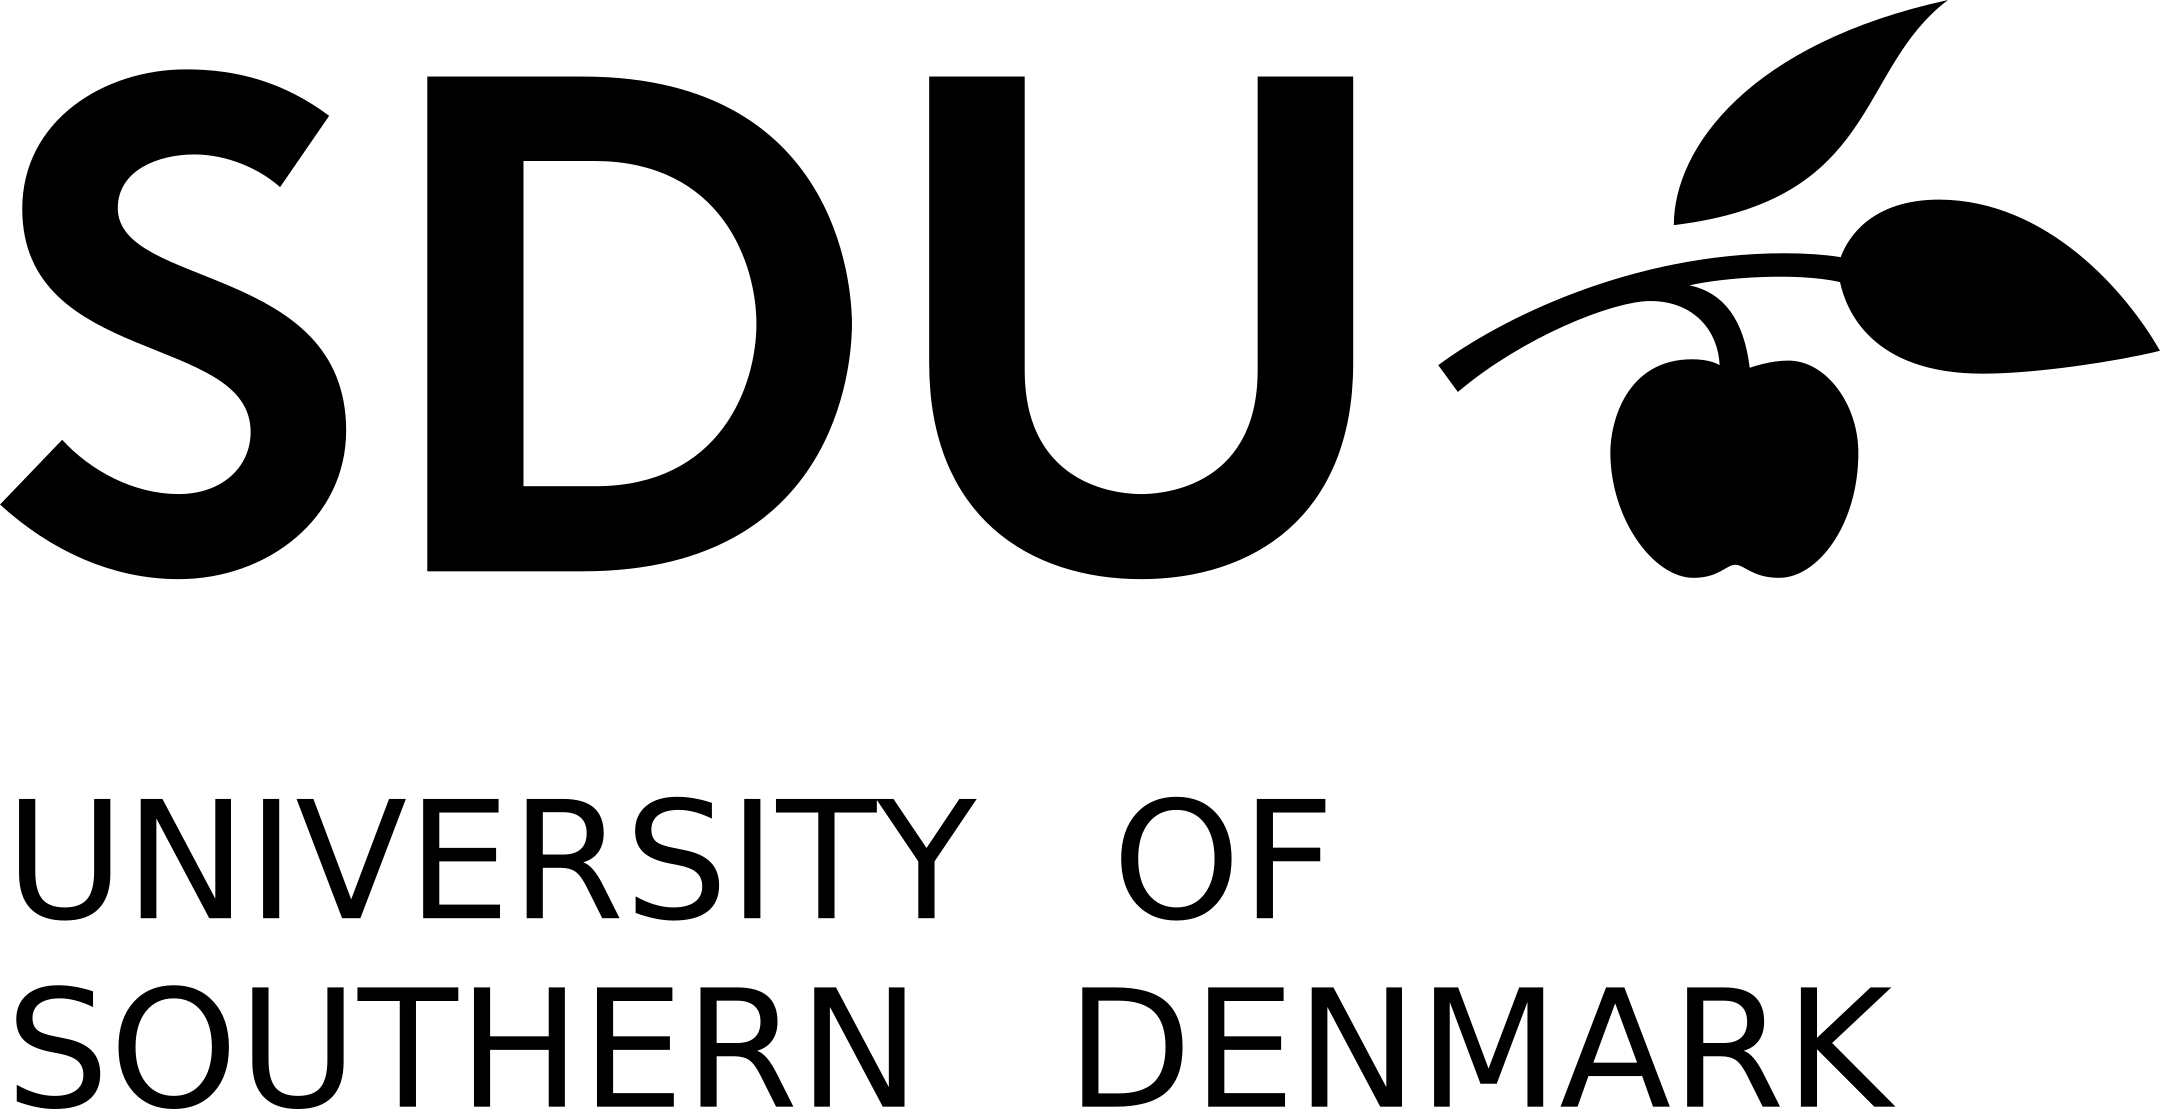
\includegraphics[scale=1]{SDU_logo}
    \vfill\ 
    \vspace{5mm}
    IMADA \\

    \textbf{\datedate}  \bf{at 10} \\[2\baselineskip]
\end{titlepage}

\renewcommand{\thepage}{\roman{page}}% Roman numerals for page counter
\tableofcontents
\newpage
\setcounter{page}{1}
\renewcommand{\thepage}{\arabic{page}}
\section{Project description}
To describe the services an operating system provides to
users, processes, and other systems\\
To discuss the various ways of structuring an operating
system\\
To explain how operating systems are installed and
customized and how they boot\\
\newpage

\section{Introduction}
This report contains documentation for the first mandatory assignment for DM818 Parallel Computing, in the first assignment we were tasked with designing a high performance singled threaded matrix matrix multiplication program.

\subsection{Work load}
For the following projected i ended up working alone as i didn't really know anyone in the course as I'm a bachelor student, the people i knew from other courses were already in groups and the remainder that i talked to were phds as were not allowed to form groups. 

\subsection{Issues}
There is currently a bug with the freeing the memory allocation, this means that the program will work one iteration. I've tried debugging with gdb and Valgrind, but i haven't been able to figure out where the bug is yet. I assume it's an overflow, or an out of place memory happening in the B Array.


\section{Design}
\subsection{Advice from lecturer}
For designing the algorithm we were given 2 examples of how its naively implemented, a naive 3 for loop implementation, and a naive blocked version. \\ \vspace{5mm}
Furthermore we were pointed heavy towards the a paper by Goto on high performance matrix multiplication, which describes how you should design the blocking for the best possible performance. \\ \vspace{5mm}
and as a third helping hand we were given a lecture by Jacob who explained how he implemented it, and what we should do to get the highest performance.
\subsection{Own design choices}

I made the design choice to follow Jacobs implementation. this meant writing functions that pack the larger matrix into smaller sub-matrices that are then used for the matrix matrix multiplication. \\
\subsubsection{Block size and Cache}
For figuring out the block size, the size of the largest possible matrix that can fit in level 2 cache was calculated.
\begin{equation}
sqr((256*1024 byte)/64 bit) = 181.019335984
\end{equation}
181 isn't a good size when handing matrix blocking, The number is therefore rounded down to nearest $2^n$ which is 128.
\begin{equation}
128 * 128 * 64 bit = 128 Kbytes
\end{equation}
An equation to solve this was also shown doing the lecture. The this is used the 128 by 128 for the main matrix, and 4 by 128 for the remaining. 
\begin{equation}
8* (m_c*k_c+m_c*n_c+N_c*k_c) = 8* (128*128+128*4+4*128) = 139264 bytes ~ 136 Kbytes
\end{equation}
After doing the calculations we can see that the program will need at least 136 KByte of cache to store the data needed. level2 cache in most modern cpu's is 256 KB, so this will suffice. A reason for not pushing it a using maybe a 256 by 128 block will mean that all 256 KB of the level2 cache would be used by the main matrix, this could cause some severed trotting issues due to it being pushed to level3 cache or main memory..\\
 
\subsubsection{Intrinsic}
I only decided on only implementing intrinsic for a core of 4x4, and just using a naive for loop implementation for the smaller blocks, as programming all the possible different blocks alone would take too much time.\\ 
\vspace{5mm}
This project was designed using avx2 instruction set, this set contains 6 data types
\begin{enumerate}
\item \_\_m128  contains 4 floats
\item \_\_m128d contains 2 doubles
\item \_\_m128i contains 8 integers
\item \_\_m256 contains 8 floats
\item \_\_m256d contains 4 doubles
\item \_\_m256i contains 16 integers
\end{enumerate}
A generalization for the naming scheme of data types is \_\_m<size><type> where size is 128, 256 or 512 when you count the newest avx512 in.
\\ \vspace{5mm}
The naming convention on the functions for the instructions follow the same scheme.
\\
\_<size>\_<name>\_<type>
Its almost the same except a few more data types can be used here. \\
The data type the project will use is pd which is packed doubles. \\
However a large array of data types are supplied to use with the intrinsic instructions.
\begin{enumerate}
\item ps  packed floats
\item pd  packed doubles
\item epi8/16/32/64 vectors containing signed integers of size 8 to 84
\item epu8/16/32/64 vectors containing unsigned integers of size 8 to 84
\item si128/si256/si512 unspecified vector of size 128, 256, or 512
\item m<size><type> when using input vectors that are different than return type.
\end{enumerate}

There are too many different functions to list so I'll only list the ones i have used in this project\\
\begin{enumerate}
\item mul - Multiplication
\item add - Adds two vectors
\item store - Stores a vector from registers to memory
\item setzero - sets all entries in a vector to 0.0
\item load - loads data from memory into registers.
\item set1 - sets all values in a vector to specified value.
\end{enumerate}
\newpage
\section{Implementation}

\subsection{Square-dgemm}

The initial function square\_dgemm gets the 3 matrices and M in as the 4 arguments. M is directly saved as a global variable. \\
3 sub matrices are then reserved, Ablock, Bblock, and C, block. Ablock and Cblock and allocated in a way that is aligned in memory by 32-bytes. this is done so the intrinsic instructions will run faster when storing or loading information. \\ \vspace{5mm}

The first for loop blocks B into blocks of of size KC * M(128 * size of matrix). The second for loop blocks A into blocks of 128 by 128 so we keep as much of A in cache as possible. \\

Prepare block is then called with the blocks we want to multiply.

\begin{lstlisting} 
void square_dgemm(int M, double *A, double *B, double *C) {
    lda = M;
    Ablock = (double *) _mm_malloc(MC * KC * sizeof(double), 32); //128*128
    Bblock = (double *) malloc(lda * KC * sizeof(double)); // M * 128
    Cblock = (double *) _mm_malloc(MC * NR * sizeof(double), 32); //128*4

    for (unsigned int k = 0; k < lda; k += KC) {
        packBBlock(B + k, std::min(KC, lda - k));
        for (unsigned int i = 0; i < lda; i += MC) {
            packAblock(A + i + k * lda, std::min(MC, lda - i), std::min(KC, lda - k));
            Prepare_block(C + i, std::min(MC, lda - i), lda, std::min(KC, lda - k));
        }
    }
    _mm_free(Ablock);
    free(Bblock);
    _mm_free(Cblock);
}
\end{lstlisting}

\subsection{Blocking functions}
The program has 2 block packing functions. and 1 unpacking, the 2 packing functions are quite close in usecase and what they do. \\
PackA packs up to 128x128 of matrix A into Ablock, and Packb packs up to 128*lda into BlockB.\\ \vspace{0mm}
The last packing function is for unblocking is for unpacking Cblock into C

\subsection{do-block}
The do block functions contains the 2 inner for loops that split A into smaller blocks, and the logic that decides if its uses the high performance multiplication function, or the naive dynamic implementation. \\
\begin{lstlisting}
void Do_block(double *C, unsigned int M, unsigned int N, unsigned int K) {
    double *B = Bblock;
    for (unsigned int n = 0; n < N; n += NR) {
        for (unsigned int m = 0; m < M; m += MR) {
            unsigned int Max_M = std::min(NR, M - m);
            unsigned int Max_N = std::min(MR, N - n);
            if (Max_M == MR && Max_N == NR) {
                core_4_4(Ablock + m * K, B, Cblock + m, K);
            } else {
                core_dyn(Ablock + m, B, Cblock +m, M, N, K);
            }
        }
        B += NR * K;
        unpackCBlock(C + n * lda, M, std::min(NR, N - n));
    }
}
\end{lstlisting}

\subsection{Core-dyn}
This is simply a stard matrix matrix multiplication function using 3 loops, and no intrinsics.

\subsection{Core-4x4}
The core 4x4 function is the high performance implementation of matrix matrix multiplication. Its performs 32 double precision floating point operations per cycle using fewer operations. \\
The first optimization that the intrinsic functions does for us is that we load 4 doubles into registers from memory at the time. \\ after this we load a single double from B into 4 positions in a vector again only using one instruction. this pattern keeps going with all out operations. we can load blocks into registers a lot faster, and we can compute 4 numbers at the time using this function.

\begin{lstlisting}
    __m256d c0 = _mm256_setzero_pd();
    __m256d a1 = _mm256_load_pd(A + k * MR);
    __m256d b00  = _mm256_set1_pd(B[k]);
    c0 = _mm256_add_pd(c0, _mm256_mul_pd(b00, a1));
    _mm256_store_pd(C, c0);
\end{lstlisting}

\section{Testing}
For testing the program i was unable to get the benchmark to work due to a memory allocation/free error in the code. i had it run once but there ware some problems 
in other parts of the code, but the performance was around 5000 mflops. but I'm currently unsure if that result could be trusted so I'm only mentioning it here.\\

The only testing I've done is to check if it returns the correct values, this was done using a testing program i made by removing some parts of the Benchmark program and changing it so it compared to the other implementations we were given as well as printing the output to the terminal for manual verification.

\section{Comparison}
The comparison of the 3 implementations we were given.
%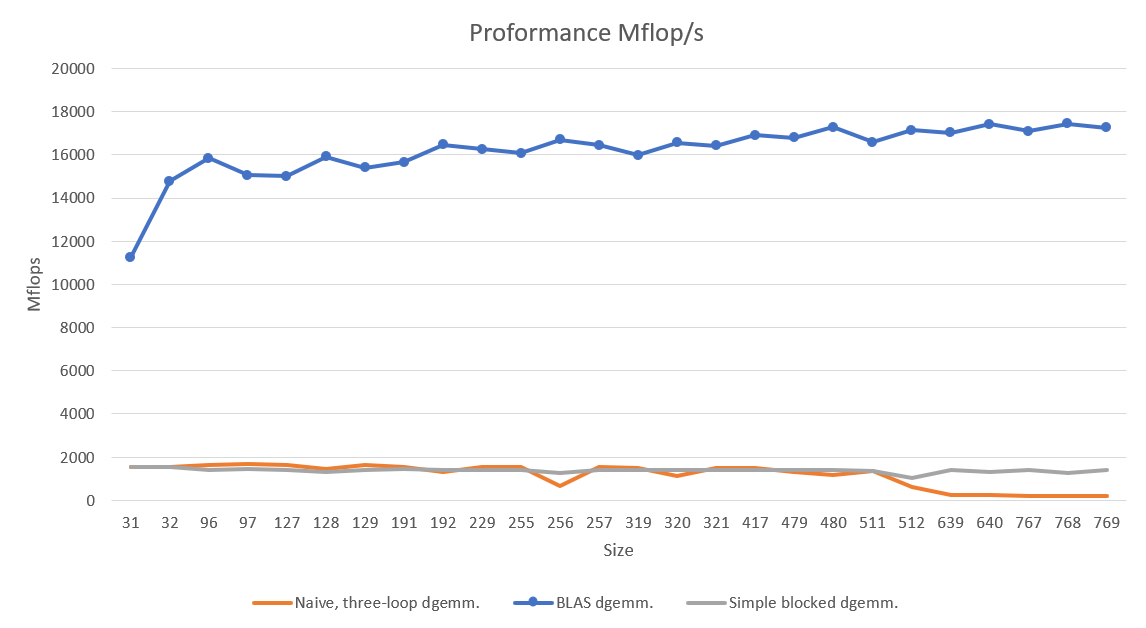
\includegraphics[scale=0.3]{mflops}


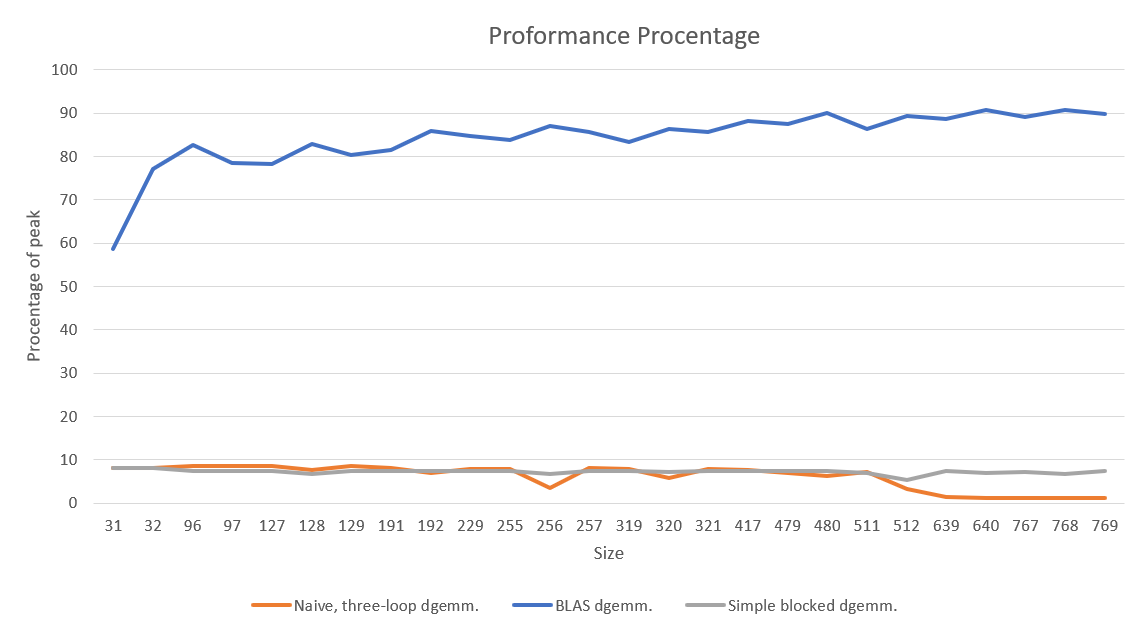
\includegraphics[scale=0.3]{Procentage}

\section{Conclusion}
The Matrix matrix multiplication assignment proved to be a bit harder than anticipated. I thought I had it working, but found out with 2 days left that there was an error i was unable to find. I did however get to learn a lot of new things, and i got to get better at using the tools for debugging and finding out where the issue in the code is. furthermore I've learned how use intrinsic and how it can boost a programs run time by a large factor.

\newpage
\section{appendix}
\subsection{Goto paper }
https://dl.acm.org/citation.cfm?id=1356053 \\
\subsection{Error, Valgrind result and stack overflow post }

\begin{lstlisting}
*** Error in `./benchmark-dgemm': munmap_chunk(): invalid pointer: 0x0000000000eca9b0 ***
benchmark-dgemm: malloc.c:2405: sysmalloc: Assertion `(old_top == initial_top (av) && old_size == 0) || ((unsigned long) (old_size) >= MINSIZE && prev_inuse (old_top) && ((unsigned long) old_end & (pagesize - 1)) == 0)' failed.


==13219== Your program just tried to execute an instruction that Valgrind
==13219== did not recognise.  There are two possible reasons for this.
==13219== 1. Your program has a bug and erroneously jumped to a non-code
==13219==    location.  If you are running Memcheck and you just saw a
==13219==    warning about a bad jump, it's probably your program's fault.
==13219== 2. The instruction is legitimate but Valgrind doesn't handle it,
==13219==    i.e. it's Valgrind's fault.  If you think this is the case or
==13219==    you are not sure, please let us know and we'll try to fix it.
==13219== Either way, Valgrind will now raise a SIGILL signal which will
==13219== probably kill your program.

https://stackoverflow.com/questions/2987207/why-do-i-get-a-c-malloc-assertion-failure
\end{lstlisting}


\section{Code}

\lstinputlisting{../src/dgemm.cpp}

%\lstinputlisting{../src/test.cpp}

\end{document}
\begin{lstlisting}
 https://software.intel.com/sites/landingpage/IntrinsicsGuide/#techs=AVX_512&cats=Elementary%20Math%20Functions,Load 
	
https://www.codeproject.com/Articles/874396/Crunching-Numbers-with-AVX-and-AVX

_mm<bit_width>_<name>_<data_type> 

The parts of this format are given as follows:

<bit_width> identifies the size of the vector returned by the function. For 128-bit vectors, this is empty. For 256-bit vectors, this is set to 256.

<name> describes the operation performed by the intrinsic
<data_type> identifies the data type of the function's primary arguments


Data Type	Description
__m128i	128-bit vector containing 8 integers
__m128	128-bit vector containing 4 floats
__m128d	128-bit vector containing 2 doubles
__m256i	256-bit vector containing 16 integers
__m256	256-bit vector containing 8 floats
__m256d	256-bit vector containing 4 doubles
__m512i	512-bit vector containing 32 integers
__m512	512-bit vector containing 16 floats
__m512d	512-bit vector containing 8 doubles



ps - vectors contain floats (ps stands for packed single-precision)
pd - vectors contain doubles (pd stands for packed double-precision)
epi8/epi16/epi32/epi64 - vectors contain 8-bit/16-bit/32-bit/64-bit signed integers
epu8/epu16/epu32/epu64 - vectors contain 8-bit/16-bit/32-bit/64-bit unsigned integers
si128/si256 - unspecified 128-bit vector or 256-bit vector
m128/m128i/m128d/m256/m256i/m256d - identifies input vector types when they're different than the type of the returned vector

\end{lstlisting}


\section{notes from lecture with Jakob}

Our cache use, calculate it to be = to 256 or maybe a bit less.
$kc and mc should be large. n_c is less important.$
kc = 128 MC = 128, 
$8* (m_c*k_c+m_c*n_c+N_c+k_c)$


$avx_256 registers are called ymm0 to 15$
$avx_512 registers are called zmm0 to 31$


Make function for each size of slices..
128 = 4.4 
256 = 8.4 
512 = 8.8


\end{document}
